% $Header: /Users/joseph/Documents/LaTeX/beamer/solutions/generic-talks/generic-ornate-15min-45min.en.tex,v 90e850259b8b 2007/01/28 20:48:30 tantau $

\documentclass{beamer}

\mode<presentation>
{
  \usetheme{Frankfurt}
  % or ...

  %\setbeamercovered{transparent}
  % or whatever (possibly just delete it)
}


\usepackage[english]{babel}
\usepackage[utf8]{inputenc}
\usepackage{times}
\usepackage[T1]{fontenc}
\usepackage{graphicx}

\title[Formalizing \emph{TAPL} in Isabelle/HOL]
{Formalizing \emph{Types and Programming Languages} in Isabelle/HOL}
\author{Martin Desharnais}
\institute[ÉTS]{École de technologie supérieure}
\date{December 10, 2014}
\subject{Talks}


% If you have a file called "university-logo-filename.xxx", where xxx
% is a graphic format that can be processed by latex or pdflatex,
% resp., then you can add a logo as follows:

%\pgfdeclareimage[height=0.5cm]{university-logo}{logo-ETS}
%\logo{\pgfuseimage{university-logo}}



% Delete this, if you do not want the table of contents to pop up at
% the beginning of each subsection:
\AtBeginSection[]
{
  \begin{frame}<beamer>{Outline}
    \tableofcontents[currentsection,currentsubsection]
  \end{frame}
}


% If you wish to uncover everything in a step-wise fashion, uncomment
% the following command:

%\beamerdefaultoverlayspecification{<+->}


\begin{document}

\begin{frame}
  \titlepage
\end{frame}

\begin{frame}{Outline}
  \tableofcontents
  % You might wish to add the option [pausesections]
\end{frame}

\section{Motivations}

\begin{frame}{Why this book?}
  \begin{columns}[c]
    \column{0.25\textwidth}
    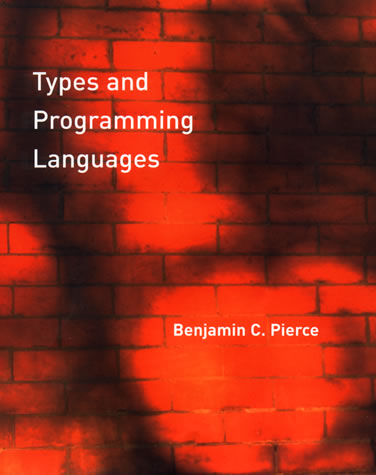
\includegraphics[scale=0.5]{TAPL.jpg} \\
    \small{Benjamin~C.~Pierce, \emph{Types and Programming Languages}, 2002}
    \column{0.75\textwidth}
    \begin{itemize}
      \item Interested in programming languages and static verification
      \item Considered as a reference on the subject
      \item Based on the mathematical foundation of $\lambda$-calculus
    \end{itemize}
  \end{columns}
\end{frame}

\begin{frame}{Why a formalization?}
  \begin{columns}[c]
    \column{0.25\textwidth}
    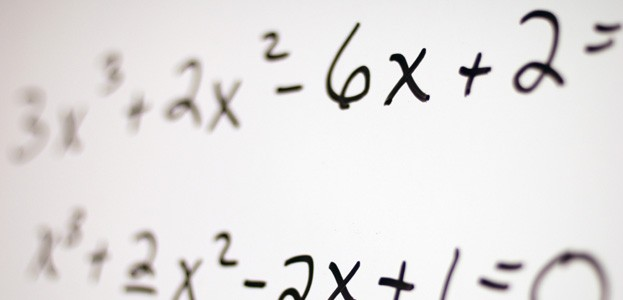
\includegraphics[scale=0.13]{whiteboard_math.jpg}
    \column{0.75\textwidth}
    \begin{definition}
       A formalization consists of definitions, properties of the defined elements and proofs that
       these properties holds.
    \end{definition}
    \begin{block}{What for?}
      \begin{itemize}
        \item Validates the pen \& paper proofs
        \item Serves as a learning tool
        \item Clarifies corner cases
      \end{itemize}
    \end{block}
  \end{columns}
\end{frame}

\begin{frame}{Why in Isabelle/HOL?}
  \begin{columns}[c]
    \column{0.25\textwidth}
    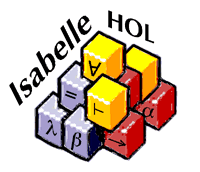
\includegraphics[scale=0.4]{isabelle_hol.png}
    \column{0.75\textwidth}
    \begin{definition}
      Isabelle/HOL is an interactive theorem prover based on Higher Order Logic.
    \end{definition}
    \begin{block}{Why this specific tool?}
      \begin{itemize}
        \item 2nd most used proof assistant \small{(behind Coq)}
        \item Took part of implementation in intership at Technische Universität München
        \item Local expertise available
      \end{itemize}
    \end{block}
  \end{columns}
\end{frame}

\section{Definition of the $\lambda$-Calculus}

\begin{frame}{What is it?}
  \begin{definition}
    The $\lambda$-calculus is a minimalist language where everything is a function.
  \end{definition}
  \begin{columns}[c]
    \footnotesize
    \column{0.4\textwidth}
    \begin{block}{$\lambda$-term}
      \begin{align}
        t & ::= \\
          & x && \text{variable} \\
          & \lambda x. \ t && \text{abstraction} \\
          & t_1 \text{ } t_2 && \text{application}
      \end{align}
    \end{block}
    \column{0.6\textwidth}
    \begin{block}{Examples}
      \begin{align*}
        & \lambda x. \ x && \text{identity} \\
        & \lambda x. \lambda y. \ x && \text{constant} \\
        & \lambda x. \lambda y. \ x \ y \ y && \text{double application} \\
        & \lambda x. \lambda y. \lambda z. \ x \ (y \ z) && \text{function composition}
      \end{align*}
    \end{block}
  \end{columns}
  \begin{description}
    \item[$\alpha$-equlivalence] Changing bound variables. \\
      $\lambda x. \ x =_\alpha \lambda y. y$
    \item[$\beta$-reduction] Applying functions to their arguments.
      $(\lambda x. \ x) y \to_\beta y$
  \end{description}
\end{frame}

\begin{frame}{How does it work?}
\end{frame}

\begin{frame}{Formalization of terms}
\end{frame}

\begin{frame}{Formalization of single-step evaluation}
\end{frame}

\begin{frame}{Formalization of multi-step evaluation}
\end{frame}

\section{Augmenting $\lambda$-Calculus with a Type System}

\begin{frame}{What are type systems?}
\end{frame}

\begin{frame}{What can type systems be used for?}
\end{frame}

\begin{frame}{Formalization of typing relation}
\end{frame}

\section{Properties of our Language}

\begin{frame}{Safety = Progress + Preservation}
\end{frame}

\begin{frame}{The progress theorem}
\end{frame}

\begin{frame}{Other theorems proved}
\end{frame}

\section*{Summary}

\begin{frame}{Summary}
\end{frame}

%\subsection[Short First Subsection Name]{First Subsection Name}

% \begin{frame}{Motivations}
%   \begin{itemize}
%     \item My personal interest on functional programming, programming languages and type systems.
%     \item My internship at TU München working on (Co)Datatypes.
%     \item Already intend to read TAPL.
%     \item Learn formalizations, Isabelle/HOL and type systems by formalizing it.
%   \end{itemize}
% \end{frame}

\end{document}


